\clearpage

\AddToShipoutPictureBG{
    \begin{tikzpicture}[remember picture, overlay]
        \node[opacity=0.04] at (current page.center) {
            
\includegraphics[width=\paperwidth,height=\paperheight]{image/fouilles}
        };
    \end{tikzpicture}
}

\chapter{Situations professionnalisantes et analyse des compétences}
\label{chap:situations_professionnalisantes}

\begin{tcolorbox}[colback=blue!6, colframe=blue!55!black, boxrule=0.5pt, arc=4pt,
  left=10pt, right=10pt, top=8pt, bottom=8pt,
  title={\textbf{\small Note de lecture : nature des situations décrites}},
  fonttitle=\small\bfseries, coltitle=white, attach boxed title to top left={yshift=-2mm, xshift=4mm},
  boxed title style={colback=blue!55!black, arc=3pt, boxrule=0pt}]
\small
Les situations professionnelles présentées dans ce chapitre sont \textbf{volontairement reconstituées et amplifiées} à des fins pédagogiques. Certains éléments contextuels (tensions, blocages, dysfonctionnements) ont été grossis ou restructurés afin de rendre visible la problématique de compétence traitée et d'en illustrer clairement les enjeux. Ces situations ne constituent pas un compte rendu factuel exhaustif des événements tels qu'ils se sont déroulés, mais un support de démonstration réflexive au service de l'analyse de compétences. L'objectif n'est pas de décrire la réalité à la virgule près, mais de mettre en lumière \textbf{ce que la formation a permis d'apprendre, et comment}.
\end{tcolorbox}

\bigskip

Chaque situation professionnelle est un gisement. En surface, elle ressemble à un événement parmi d'autres : une réunion difficile, un choix technique à trancher, un processus à faire évoluer. C'est le travail de fouille qui en révèle la valeur : creuser sous l'anecdote pour dégager les strates d'apprentissage, tamiser les matériaux accumulés pour en extraire les traces significatives, et mettre au jour les artefacts\footnote{Un \textbf{artefact} désigne un document, un outil ou un livrable produit pendant l'action. Dans ce chapitre, il sert de preuve observable de la compétence mobilisée.} qui, une fois exhumés et analysés, attestent d'une transformation réelle. Ce chapitre est le compte rendu de trois fouilles. Pour chacune des compétences retenues, il documente ce qui a été sondé, ce qui a été extrait, et ce que la profondeur atteinte révèle sur le chemin parcouru.

% ==============================================================================
\section{Compétence A2 : Anticiper et gérer les divergences}
\label{sec:competence-a2}
% ==============================================================================

\begin{tcolorbox}[colback=gray!5, colframe=gray!40, boxrule=0.4pt, arc=3pt,
  left=8pt, right=8pt, top=6pt, bottom=6pt]
\small\itshape
\textbf{Définition (référentiel Innokick, Phase Définition).}
Anticiper et gérer les divergences afin de faciliter un processus participatif de convergence en intégrant les préconceptions, les besoins et les enjeux des différents acteurs à l'aide de méthodes agiles\footnotemark, de méthodes de communication et de médiation\footnotemark.
\end{tcolorbox}
\addtocounter{footnote}{-2}%
\addtocounter{footnote}{1}\footnotetext{Les \textbf{méthodes agiles} désignent des approches de projet fondées sur des cycles courts, la collaboration et l'adaptation continue. Elles privilégient des livraisons incrémentales plutôt qu'une planification figée.}%
\addtocounter{footnote}{1}\footnotetext{La \textbf{médiation} désigne un processus structuré où un tiers neutre aide deux parties à converger sans imposer de décision. Elle se distingue de l'arbitrage, où la décision est tranchée par une autorité.}

\bigskip

\bigskip

% : A2.1 : Autoévaluation ---
\subsection{Autoévaluation de ma progression}


Parmi toutes les compétences sondées durant la formation, A2 est celle dont la fouille a mis au jour les strates les plus inattendues. En surface, je savais gérer un désaccord : bon sens, expérience, intuition sociale. Mais en creusant, la formation a révélé que je ne disposais d'aucun protocole pour transformer une divergence en convergence structurée. Mon score auto-évalué reflète cette excavation : la couche supérieure était déjà présente à l'entrée en formation ; c'est la profondeur, la capacité à opérer avec méthode et reproductibilité, qui a été véritablement dégagée.

% : A2.2 : Situation et preuves ---
\subsection{Situation professionnalisante et preuves}

\subsubsection*{La situation}

La première scène (\textbf{avant la formation}) se déroule dans le département reporting\footnote{Le \textbf{reporting} financier désigne la production périodique de rapports destinés aux clients d'une institution financière. Ces rapports synthétisent notamment la performance, les risques et, selon les cas, les indicateurs ESG.} d'une banque privée. L'équipe doit faire évoluer un outil de génération de rapports clients : le processus actuel est trop coûteux en heures et la direction demande une optimisation. Plusieurs options techniques existent : automatiser davantage avec des outils internes, adopter un outil tiers, ou refondre le processus en standardisant les templates\footnote{Un \textbf{template} (gabarit) désigne un modèle réutilisable qui standardise la structure d'un document. Son usage réduit le temps de production et les écarts de forme entre livrables.}. Les discussions tournent vite au débat de positions\footnote{En négociation, une \textbf{position} décrit ce qu'un acteur demande, alors qu'un \textbf{intérêt} décrit la raison sous-jacente de cette demande. Travailler sur les intérêts facilite la convergence, même lorsque les positions s'opposent.}, sans critères partagés ni arbitrage explicite.

Dans cette strate \textit{avant}, plusieurs éléments manquaient : aucun cadrage temporel de la discussion, aucun protocole de comparaison des options, aucune pondération collective des critères, et aucun artefact final consignant le raisonnement. En fouille, cela se traduit par un sous-sol pauvre : beaucoup de parole, peu de traces, et donc peu de capacité à défendre la décision face au management ou à la reprendre quelques mois plus tard.

La seconde scène (\textbf{après la formation}) se déroule chez TWIICE : même type de divergence collective, mais avec une posture transformée par la formation. Les désaccords sur la traçabilité SOUP\footnote{\textbf{SOUP} (\emph{Software of Unknown Provenance}) désigne des composants logiciels tiers non développés en interne. En contexte médical, leur suivi (version, origine, risque, licence) est requis par IEC~62304.} et les choix d'outillage\footnote{L'\textbf{outillage} désigne l'ensemble des outils de développement et de pilotage : gestion de code, suivi des tâches, intégration continue, génération d'artefacts et documentation.} sont traités selon une séquence explicite : recadrage de l'objectif commun, priorisation des enjeux, comparaison multicritère, puis formalisation écrite de la décision.

Le bénéfice n'est pas seulement décisionnel ; il est aussi documentaire et collectif. Là où la banque laissait des traces éparses, TWIICE produit des artefacts reliés entre eux (note de décision, backlog\footnote{Le \textbf{backlog} désigne la liste priorisée des tâches, demandes et évolutions d'un projet. Il est mis à jour en continu selon les apprentissages et les contraintes.} priorisé, mapping Eisenhower), ce qui rend la convergence vérifiable, transmissible et réutilisable dans les sprints suivants. La divergence n'est plus un bruit de fond : elle devient une matière première traitée avec méthode.

\subsubsection*{Les trois artefacts exhumés}

\paragraph{Preuve 1 : Banque privée (avant) : contre-exemple et traces limitées}

La situation bancaire est conservée comme \textbf{carotte témoin} de la fouille : elle montre précisément ce qui manque quand la compétence A2 n'est pas instrumentée. Concrètement, la discussion avançait en séquences d'arguments individuels, sans phase explicite de synthèse ni critères de comparaison. Les options étaient évoquées, mais jamais scorées ; les contraintes client étaient citées, mais pas traduites en critères partagés.

Résultat observable : après deux réunions, aucun arbitrage robuste\footnote{Une \textbf{chaîne de décision robuste} relie de manière explicite le problème initial, les options évaluées, les critères, la décision et ses effets observables. Elle rend la décision compréhensible et réutilisable.}, aucune responsabilité formalisée, et donc un retour périodique du même débat. Cette pauvreté de traces n'est pas un détail rédactionnel : c'est la preuve négative qui met en évidence ce que la formation a ensuite apporté.

\paragraph{Preuve 2 : TWIICE (après) : note de décision technique formalisée}

L'Annexe~\ref{annex:ndt-sw-001} constitue la \textbf{preuve centrale} de l'après-formation : on y voit comment la divergence a été convertie en convergence. La méthode utilisée est explicite :

\begin{itemize}
  \item \textbf{Étape 1 : recadrage du problème} : la discussion ne porte plus sur « l'outil préféré », mais sur l'exigence normative prioritaire (traçabilité IEC~62304).
  \item \textbf{Étape 2 : explicitation des options} : GitLab, solution custom, JFrog sont posés à plat dans un même périmètre de comparaison.
  \item \textbf{Étape 3 : grille multicritère partagée} : coût, délai, intégration, dépendance fournisseur, cybersécurité, conformité ; les options sont comparées avec une logique commune\footnote{Une \textbf{analyse multicritère} compare plusieurs options au regard de critères explicites (coût, délai, risque, conformité, etc.), souvent pondérés. Elle permet de justifier un arbitrage de manière transparente.}.
  \item \textbf{Étape 4 : décision + risques résiduels} : la décision est prise, mais aussi encadrée par des mesures de mitigation, ce qui la rend défendable en audit\footnote{Une décision \textbf{auditable} est une décision dont les preuves (données, critères, arbitrages, validations) permettent une vérification externe ultérieure.}.
\end{itemize}

Le gain n'est pas déclaratif : le document permet de reconstruire tout le raisonnement, de vérifier les arbitrages et d'aligner équipe logicielle et qualité sur une base commune.

\paragraph{Preuve 3 : TWIICE (après) : traçabilité opérationnelle dans le backlog}

L'Annexe~\ref{annex:backlog} montre la phase d'extraction la plus importante : la décision n'est pas restée théorique, elle a été traduite en travail exécutable. Les items liés à la certification passent en priorité HIGH, les sujets non bloquants sont déplacés hors du sprint critique, et chaque ticket est rattaché à une logique importance/urgence (quadrants Eisenhower\footnote{La \textbf{matrice d'Eisenhower} classe les sujets selon deux axes : importance et urgence. Elle permet de distinguer ce qui doit être traité immédiatement de ce qui peut être planifié, délégué ou reporté.}).

Cette preuve documente le mécanisme causal attendu pour A2 :

\begin{itemize}
  \item sans méthode (banque) : divergence prolongée, décisions implicites, traces faibles ;
  \item avec méthode (TWIICE) : divergence cadrée, arbitrage explicite, priorisation visible, exécution suivie.
\end{itemize}

Autrement dit, la formation n'a pas seulement amélioré la qualité du débat ; elle a amélioré la qualité des résultats produits par ce débat.

% : A2.3 : Ressources ---
\subsection{Ressources mobilisées et combinées}

Les ressources mobilisées dans cette fouille A2 sont de trois ordres.

\textbf{1) Ressources de posture.}
La distinction positions/intérêts, travaillée en formation, a servi d'outil de décantation : quand une discussion se figeait sur « quelle solution ? », je reformulais en « quel besoin critique cherchons-nous à sécuriser ? ». Ce déplacement de registre a permis de diminuer la charge défensive des échanges et de rouvrir la possibilité de convergence.

\textbf{2) Ressources de méthode.}
Le timeboxing\footnote{Le \textbf{timeboxing} désigne l'attribution d'une durée fixe et non extensible à une activité. En facilitation, il évite l'enlisement et force la production d'un résultat dans le temps imparti.}, la grille de critères et le vote par points\footnote{Le \textbf{vote par points} désigne une méthode de sélection collective où chaque participant dispose d'un nombre limité de votes. La convergence s'appuie sur une agrégation des préférences du groupe.} ont été utilisés comme tamis successifs : d'abord borner la discussion, ensuite comparer sur des bases communes, enfin trancher collectivement sans personnaliser l'arbitrage.

\textbf{3) Ressources de facilitation.}
Le recadrage prosodique\footnote{Le \textbf{recadrage prosodique} désigne une intervention sur le ton et le registre d'un échange pour le ramener vers l'objectif commun. Il aide à passer d'un débat d'opinions à un débat fondé sur des critères.} a servi à ramener le groupe d'un registre d'affirmation (« je pense que... ») vers un registre de preuve (« sur quel critère objectif s'appuie cette option ? »). C'est cette combinaison posture + méthode + facilitation qui explique la différence entre le gisement pauvre de la banque et les artefacts exploitables de TWIICE.

% : A2.4 : Analyse réflexive ---
\subsection{Analyse réflexive}

La lecture croisée des deux scènes confirme que la divergence n'était jamais le problème principal. Le problème était l'absence d'outils pour traiter cette divergence. À la banque, l'énergie du groupe restait en surface, dans des échanges d'autorité ; à TWIICE, la même énergie a pu être canalisée vers des artefacts de décision.

Le point de bascule le plus important est méthodologique : je ne cherche plus à « convaincre mieux », je cherche à \textit{structurer mieux}. Cette posture change la nature de ma contribution. Je ne suis plus uniquement la voix d'une option technique ; je deviens l'architecte du processus de convergence. C'est précisément ce que la compétence A2 exige.

Enfin, cette fouille révèle une leçon durable : la facilitation\footnote{La \textbf{facilitation} désigne l'ensemble des pratiques qui structurent le travail collectif vers un objectif commun. Le facilitateur organise le processus et la parole, sans décider à la place du groupe.} n'est pas un talent spontané, c'est une discipline outillée. Lorsqu'elle est préparée, les traces produites sont plus profondes, plus fiables et plus utiles que la mémoire des échanges.

% : A2.5 : Apprentissages à entreprendre ---
\subsection{Apprentissages à entreprendre}

Trois apprentissages sont à poursuivre pour approfondir cette compétence.

\textbf{1) Ritualiser le protocole de convergence.}
Formaliser un canevas réutilisable (objectif, critères, options, décision, risques) pour éviter de reconstruire la méthode à chaque nouveau désaccord.

\textbf{2) Mieux instrumenter la transition opinions -> données.}
Introduire systématiquement un support visuel de critères dès les premières minutes d'une réunion sensible, afin de réduire la polarisation des positions.

\textbf{3) Renforcer la traçabilité des arbitrages.}
Produire après chaque décision un artefact court mais complet (raisonnement, options écartées, critères, responsables, échéances) pour consolider la mémoire collective et faciliter les audits internes.

% ==============================================================================
\section{Compétence B4 : Méthodes agiles au service du prototypage itératif}
\label{sec:competence-b4}
% ==============================================================================

\begin{tcolorbox}[colback=gray!5, colframe=gray!40, boxrule=0.4pt, arc=3pt,
  left=8pt, right=8pt, top=6pt, bottom=6pt]
\small\itshape
\textbf{Définition (référentiel Innokick, Phase Prototypage).}
Choisir et mettre en œuvre des méthodes agiles, telle que la méthode lean\footnotemark, favorisant la réalisation de prototypes\footnotemark, de manière itérative\footnotemark, dans le but de créer un maximum de valeur en optimisant les ressources disponibles.
\end{tcolorbox}
\addtocounter{footnote}{-3}%
\addtocounter{footnote}{1}\footnotetext{La \textbf{méthode lean} désigne une approche visant à maximiser la valeur produite tout en réduisant les gaspillages. En logiciel, elle privilégie des incréments utiles et rapides plutôt que des livraisons monolithiques.}%
\addtocounter{footnote}{1}\footnotetext{Un \textbf{prototype} désigne une version partielle d'un produit destinée à tester une hypothèse de conception ou un besoin utilisateur. Son niveau de fidélité varie selon l'objectif du test.}%
\addtocounter{footnote}{1}\footnotetext{Une démarche \textbf{itérative} procède par cycles successifs produisant des livrables testables. Chaque cycle intègre des retours pour ajuster le suivant.}

\bigskip

% : B4.1 : Autoévaluation ---
\subsection{Autoévaluation de ma progression}


La fouille de cette compétence a révélé un paradoxe : le gisement existait déjà, mais restait inexploité. Je pratiquais des itérations courtes depuis plusieurs années. Ce que la formation a mis au jour, c'est l'épaisseur de ce que je ne savais pas faire : adapter la méthode à un terrain réglementé, articuler agilité et traçabilité sans sacrifier l'une à l'autre. Les sédiments de la certification médicale (IEC~62304\footnote{L'\textbf{IEC~62304} désigne la norme qui encadre le cycle de vie des logiciels de dispositifs médicaux. Elle impose des exigences de traçabilité, de documentation et de maîtrise des risques, avec des classes de sécurité A, B et C.}) rendaient le sol difficile à sonder ; la formation m'a fourni les instruments pour en extraire quelque chose d'utilisable.

% : B4.2 : Situation et preuves ---
\subsection{Situation professionnalisante et preuves}

\subsubsection*{La situation}

Chez TWIICE\footnote{\textbf{TWIICE} désigne une entreprise suisse développant des exosquelettes médicaux pour la rééducation motrice.}, le développement logiciel de l'exosquelette\footnote{Un \textbf{exosquelette médical} désigne un dispositif mécatronique portable qui assiste ou remplace la motricité. En rééducation, il guide les mouvements pour soutenir la reprise de la marche.} suivait jusqu'alors une logique séquentielle : concevoir en entier, développer en entier, tester en entier, certifier. Ce modèle dit \emph{en cascade}\footnote{Le développement \textbf{en cascade} (\emph{waterfall}) désigne une approche séquentielle où chaque phase est clôturée avant la suivante. Son principal risque est de découvrir les erreurs tardivement, quand leur correction devient coûteuse.} donne une impression rassurante de maîtrise : chaque phase semble bouclée avant de passer à la suivante. En pratique, les erreurs de conception ne se révèlent que lors des tests finaux, plusieurs mois après avoir été commises, à un moment où les corriger coûte cher en temps et en documentation.

L'enjeu était d'introduire une logique itérative : des cycles courts (deux semaines), des livrables partiels mais testables à chaque sprint\footnote{Un \textbf{sprint} désigne une période de travail courte et fixe, au terme de laquelle l'équipe livre un incrément testable. C'est l'unité de base de Scrum.}, et des rétrospectives\footnote{Une \textbf{rétrospective} désigne la réunion de fin de sprint où l'équipe analyse ce qui a fonctionné, ce qui a bloqué et les actions à mettre en place. Elle alimente l'amélioration continue.} permettant d'apprendre en chemin. La résistance de l'équipe qualité était légitime et formulée clairement : \emph{« Comment certifier quelque chose qu'on change en permanence ? »} Cette tension entre la culture de l'agilité (accepter le changement, livrer vite, itérer) et les exigences de la certification médicale (tout documenter, tout tracer, tout valider) est le nœud central de cette compétence.

La réponse apportée n'a pas consisté à choisir l'un ou l'autre, mais à montrer que la contradiction est fausse : une approche itérative bien outillée produit des preuves de certification plus granulaires et plus fiables qu'un développement monolithique, à condition d'intégrer les exigences documentaires directement dans la \textit{Definition of Done}\footnote{La \textbf{Definition of Done} désigne l'ensemble des critères qu'un livrable doit satisfaire pour être considéré comme terminé. En contexte médical, elle inclut le code, les tests, la documentation et la validation qualité.} de chaque sprint.

\subsubsection*{Les trois artefacts exhumés}

\medskip\noindent\textbf{Preuve 1 : Proposition de découpage en sprints adaptée IEC~62304}\par\smallskip

\begin{acompleter}{Preuve 1 B4 : à reconstituer}
Reconstituer le document interne présentant la structure sprint de 2 semaines : objectifs du sprint, livrables attendus, Definition of Done adaptée (code + tests + documentation IEC~62304 + revue qualité + archivage GitLab\footnote{\textbf{GitLab} désigne une plateforme de gestion de code et de collaboration intégrant suivi des tâches et pipelines CI/CD. Dans ce projet, elle sert de support principal de traçabilité du développement.}), et le tableau de correspondance entre les livrables de sprint et les enregistrements requis par la norme. Ce document a été présenté à l'équipe qualité pour démontrer que l'agilité et la traçabilité réglementaire sont compatibles.
\end{acompleter}

\medskip\noindent\textbf{Preuve 2 : Backlog\footnotemark{} priorisé du premier trimestre (Annexe~\ref{annex:backlog})}\par\smallskip
\footnotetext{Le \textbf{backlog} désigne la liste priorisée de tout ce qu'il reste à réaliser dans un projet. Il est actualisé en continu au fil des sprints.}

L'artefact central de cette compétence est reproduit en intégralité en Annexe~\ref{annex:backlog}. Il s'agit d'un extrait du board\footnote{Un \textbf{board} agile désigne une représentation visuelle des tâches d'un projet, généralement structurée en colonnes (À faire / En cours / Terminé). Il donne une vue immédiate de l'avancement et des blocages.} GitLab de l'équipe TWIICE, exporté après l'application de la grille de priorisation par \emph{valeur fonctionnelle $\times$ risque certification}. Chaque item est classifié par niveau de priorité (HIGH, MEDIUM, LOW) et tracé jusqu'au quadrant Eisenhower\footnote{La \textbf{matrice d'Eisenhower} (importance/urgence) classe les tâches selon leur impact et leur délai. Elle sert à distinguer ce qui doit être traité immédiatement de ce qui peut être planifié ou reporté.} correspondant. Ce backlog documente le passage d'une liste de débats parallèles à une file de travail ordonnée et actionnable, dans laquelle les sujets bloquants pour la certification ont été remontés en tête de sprint.

\paragraph{Preuve 3 : Compte-rendu de la première rétrospective d'équipe}

\begin{acompleter}{Preuve 3 B4 : à reconstituer}
Reconstituer le CR de la première rétrospective (format Start/Stop/Continue\footnote{Le format \textbf{Start / Stop / Continue} désigne un cadre de rétrospective en trois volets : ce qu'on commence, ce qu'on arrête, ce qu'on poursuit. Il transforme le bilan en plan d'action concret.}) tenue après le premier sprint complet. Le document doit contenir : les points qui ont fonctionné (Continue), les pratiques à abandonner (Stop), et les trois actions d'amélioration retenues pour le sprint suivant (Start). Ce CR documente la capacité d'apprentissage en cours de processus : non pas la perfection du premier sprint, mais la volonté d'ajuster méthodiquement.
\end{acompleter}

% : B4.3 : Ressources ---
\subsection{Ressources mobilisées et combinées}

\begin{acompleter}{Ressources B4}
Rédiger ici les ressources de façon autonome. À couvrir : (1) Scrum\footnotemark{} : le cycle sprint-revue-rétrospective comme boucle d'apprentissage (Sutherland, 2014) ; (2) la Definition of Done comme contrat qualité interne, et son adaptation aux exigences IEC~62304 (code + tests + doc + revue) ; (3) la priorisation backlog par valeur fonctionnelle × risque certification : justifier pourquoi ce double critère est indispensable dans un contexte médical ; (4) la rétrospective comme moteur d'amélioration continue : le format Start/Stop/Continue et son usage en équipe pluridisciplinaire\footnotemark.
\end{acompleter}
% 2 footnotes dans la boîte ci-dessus — compteur remis en position correcte
\addtocounter{footnote}{-2}%
\addtocounter{footnote}{1}\footnotetext{\textbf{Scrum} désigne un cadre agile structuré autour de sprints, de rôles définis et de cérémonies régulières (planification, revue, rétrospective). Il organise la livraison incrémentale et l'apprentissage d'équipe.}%
\addtocounter{footnote}{1}\footnotetext{Une \textbf{équipe pluridisciplinaire} désigne un collectif réunissant des expertises différentes. Cette diversité augmente la richesse des solutions, mais demande un effort explicite d'alignement.}

% : B4.4 : Analyse réflexive ---
\subsection{Analyse réflexive}

\begin{acompleter}{Analyse réflexive B4}
Rédiger ici l'analyse de façon autonome. Points à développer : (1) l'opposition agilité / certification est fausse : une approche itérative bien documentée produit des preuves plus granulaires et plus défendables qu'un développement monolithique, car les erreurs sont découvertes et corrigées tôt ; (2) la résistance de l'équipe qualité n'était pas irrationnelle : elle reflétait une expérience réelle de projets agiles sans discipline documentaire ; convaincre demandait de montrer, pas d'affirmer ; (3) ce qui a changé dans ma posture : ne plus subir la certification comme une contrainte externe mais la traiter comme un critère de conception à intégrer dès le sprint planning\footnote{Le \textbf{sprint planning} désigne la réunion d'ouverture du sprint durant laquelle l'équipe sélectionne les éléments du backlog et planifie le travail. C'est le moment clé pour intégrer les exigences qualité et réglementaires.}.
\end{acompleter}

% : B4.5 : Apprentissages à entreprendre ---
\subsection{Apprentissages à entreprendre}

\begin{acompleter}{Apprentissages B4}
Reprendre et actualiser les apprentissages identifiés dans le journal réflexif (section B4, §5) : frameworks agile certifiables pour dispositifs médicaux (SAFe for Medical\footnote{\textbf{SAFe for Medical} (\emph{Scaled Agile Framework for Medical Devices}) désigne une adaptation de SAFe aux contraintes réglementaires du médical. Il propose des pratiques conciliant cadence agile et traçabilité normative.}), Definition of Done standard, pratique des rétrospectives.
\end{acompleter}

% ==============================================================================
\section{Compétence C2 : Synthèse et définition des problématiques prioritaires}
\label{sec:competence-c2}
% ==============================================================================

\begin{tcolorbox}[colback=gray!5, colframe=gray!40, boxrule=0.4pt, arc=3pt,
  left=8pt, right=8pt, top=6pt, bottom=6pt]
\small\itshape
\textbf{Définition (référentiel Innokick, Phase Définition).}
Synthétiser les informations recueillies dans la phase d'empathie\footnotemark{} pour définir des problématiques à résoudre et/ou des opportunités à développer.
\end{tcolorbox}
\footnotetext{La \textbf{phase d'empathie} désigne la première étape du Design Thinking. Elle vise à comprendre les utilisateurs avant de formuler un problème ou une solution.}

\bigskip

% : C2.1 : Autoévaluation ---
\subsection{Autoévaluation de ma progression}


C'est le gisement le mieux documenté des trois fouilles. La formation a mis au jour quelque chose de précis : ma tendance à me précipiter vers les solutions sans avoir d'abord bien cerné le problème. Les outils de définition de problème et de priorisation\footnote{La \textbf{priorisation} désigne le classement explicite d'éléments selon leur importance, urgence ou valeur. Elle permet de concentrer l'effort sur les actions les plus impactantes.} ont permis de structurer ma réflexion et d'éviter les solutions hâtives. La profondeur de la fouille a également été limitée par ma méconnaissance des méthodes de recherche utilisateur\footnote{Les \textbf{méthodes de recherche utilisateur} désignent les techniques permettant de comprendre besoins, usages et motivations des utilisateurs. Elles combinent généralement approches qualitatives et quantitatives.}.

% : C2.2 : Situation et preuves ---
\subsection{Situation professionnalisante et preuves}

\subsubsection*{La situation}

Dans le cadre de mes fonctions chez TWIICE, j'ai été confronté à un défi récurrent : comment prioriser les évolutions à apporter à notre exosquelette en fonction des retours utilisateurs et des contraintes techniques ? Les demandes d'amélioration provenaient à la fois des utilisateurs finaux (patients, thérapeutes) et des équipes internes (ingénierie, qualité, réglementation). Chacun avait ses propres priorités, souvent divergentes.

Une première approche a consisté à rassembler toutes les demandes dans une liste unique, sans distinction ni hiérarchisation. Rapidement, cette liste est devenue ingérable : plus de 150 items hétérogènes, allant de la simple suggestion d'amélioration à des demandes complexes nécessitant des études de faisabilité. Les réunions pour en discuter se terminaient systématiquement par des frustrations, chaque partie campant sur ses positions sans parvenir à un accord.

Il est vite apparu que cette méthode, ou plutôt ce manque de méthode, générait plus de conflits que de solutions. L'absence de critères clairs pour évaluer et prioriser les demandes conduisait à des débats stériles et à une paralysie décisionnelle. Il était urgent de trouver un cadre commun permettant d'aligner les différentes parties prenantes sur des priorités partagées.

\subsubsection*{Les trois artefacts exhumés}

\paragraph{Preuve 1 : Matrice de priorisation des évolutions}

\begin{acompleter}{Preuve 1 C2 : à reconstituer}
Produire la matrice de priorisation utilisée pour classer les demandes d'évolutions selon deux axes : l'impact potentiel sur l'utilisateur (élevé, moyen, faible) et la faisabilité technique (facile, moyen, difficile). Cette matrice a permis d'objectiver les discussions en se basant sur des critères communs et visibles par tous.
\end{acompleter}

\paragraph{Preuve 2 : Compte-rendu de l'atelier de définition des problématiques}

\begin{acompleter}{Preuve 2 C2 : à reconstituer}
Rédiger le CR d'un atelier réunissant les principales parties prenantes (utilisateurs, ingénieurs, qualité) visant à définir collectivement les 3 à 5 problématiques prioritaires à résoudre. Le document doit retracer les échanges, les points de vue divergents, et comment ils ont été intégrés dans la problématique finale.
\end{acompleter}

\paragraph{Preuve 3 : Feuille de route des évolutions}

\begin{acompleter}{Preuve 3 C2 : à reconstituer}
Produire la feuille de route actualisée des évolutions du produit, intégrant les problématiques prioritaires définies, les objectifs associés, et les indicateurs de succès. Ce document sert de guide pour les développements futurs et de contrat d'objectifs entre les équipes.
\end{acompleter}

% : C2.3 : Ressources ---
\subsection{Ressources mobilisées et combinées}

\begin{acompleter}{Ressources C2}
Rédiger ici les ressources de façon autonome. À couvrir : (1) la définition et l'importance de la phase d'empathie dans le Design Thinking (Brown, 2009) ; (2) les méthodes de recherche utilisateur : entretiens, questionnaires, observations, et comment en tirer des insights exploitables ; (3) la priorisation par la matrice d'Eisenhower et la méthode MoSCoW (Must, Should, Could, Won't) ; (4) l'animation d'ateliers de co-création avec des parties prenantes pluridisciplinaires.
\end{acompleter}

% : C2.4 : Analyse réflexive ---
\subsection{Analyse réflexive}

\begin{acompleter}{Analyse réflexive C2}
Rédiger ici l'analyse de façon autonome. Points à développer : (1) l'importance cruciale de la phase d'empathie pour éviter les solutions imposées et déconnectées des besoins réels ; (2) comment la matrice de priorisation a transformé notre approche : passer d'une liste de souhaits à une feuille de route stratégique ; (3) les enseignements tirés sur la gestion des parties prenantes : impliquer en amont pour éviter les résistances et favoriser l'adhésion.
\end{acompleter}

% : C2.5 : Apprentissages à entreprendre ---
\subsection{Apprentissages à entreprendre}

\begin{acompleter}{Apprentissages C2}
Reprendre et actualiser les apprentissages identifiés dans le journal réflexif (section C2, §5) : approfondir les méthodes de recherche utilisateur, s'entraîner à l'animation d'ateliers, expérimenter la priorisation par la valeur et le risque.
\end{acompleter}


% ==============================================================================
\section{Bilan de progression : vue d'ensemble}
\label{sec:bilan-progression}
% ==============================================================================

Les trois radars ci-dessous restituent l'évolution auto-évaluée sur chacune des familles de compétences (A, B, C). Les tableaux associés précisent pour chaque dimension le score estimé avant et après la formation, ainsi que la justification de l'autoévaluation initiale. Ces données sont à lire comme des \emph{instantanés réflexifs}, non comme des mesures objectives.

% -----------------------------------------------------------------------
% RADARS
% -----------------------------------------------------------------------
\begin{figure}[ht]
\centering
% ---- Radar famille A ----
\begin{minipage}[t]{0.32\textwidth}
\centering
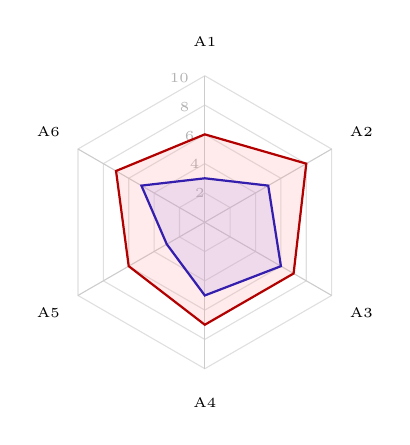
\begin{tikzpicture}[scale=0.62]
\pgfmathsetmacro{\R}{3}
\foreach \r in {0.6,1.2,1.8,2.4,3.0}{
  \draw[gray!25](90:\r)--(30:\r)--(-30:\r)--(-90:\r)--(-150:\r)--(150:\r)--cycle;}
\foreach \r/\v in {0.6/2,1.2/4,1.8/6,2.4/8,3.0/10}{
  \node[gray!60,font=\tiny] at (100:\r) {\v};}
\draw[gray!40](0,0)--(90:\R);
\draw[gray!40](0,0)--(30:\R);
\draw[gray!40](0,0)--(-30:\R);
\draw[gray!40](0,0)--(-90:\R);
\draw[gray!40](0,0)--(-150:\R);
\draw[gray!40](0,0)--(150:\R);
\node[font=\tiny] at (90:3.7)  {A1};
\node[font=\tiny] at (30:3.7)  {A2};
\node[font=\tiny] at (-30:3.7) {A3};
\node[font=\tiny] at (-90:3.7) {A4};
\node[font=\tiny] at (-150:3.7){A5};
\node[font=\tiny] at (150:3.7) {A6};
\draw[thick,blue!70!black,fill=blue!40,fill opacity=0.20]
  (90:0.9)--(30:1.5)--(-30:1.8)--(-90:1.5)--(-150:0.9)--(150:1.5)--cycle;
\draw[thick,red!70!black,fill=red!40,fill opacity=0.20]
  (90:1.8)--(30:2.4)--(-30:2.1)--(-90:2.1)--(-150:1.8)--(150:2.1)--cycle;
\end{tikzpicture}
\par\smallskip{\small\textbf{Famille A}}\par{\footnotesize Compétences sociales et personnelles}
\end{minipage}
\hfill
% ---- Radar famille B ----
\begin{minipage}[t]{0.32\textwidth}
\centering
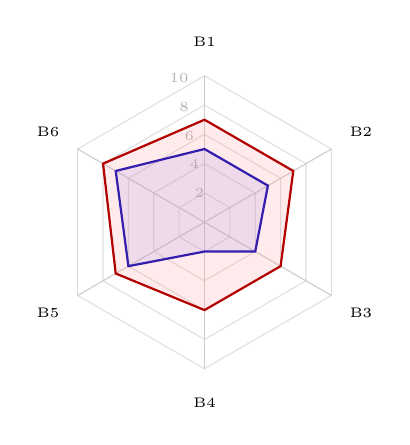
\begin{tikzpicture}[scale=0.62]
\pgfmathsetmacro{\R}{3}
\foreach \r in {0.6,1.2,1.8,2.4,3.0}{
  \draw[gray!25](90:\r)--(30:\r)--(-30:\r)--(-90:\r)--(-150:\r)--(150:\r)--cycle;}
\foreach \r/\v in {0.6/2,1.2/4,1.8/6,2.4/8,3.0/10}{
  \node[gray!60,font=\tiny] at (100:\r) {\v};}
\draw[gray!40](0,0)--(90:\R);
\draw[gray!40](0,0)--(30:\R);
\draw[gray!40](0,0)--(-30:\R);
\draw[gray!40](0,0)--(-90:\R);
\draw[gray!40](0,0)--(-150:\R);
\draw[gray!40](0,0)--(150:\R);
\node[font=\tiny] at (90:3.7)  {B1};
\node[font=\tiny] at (30:3.7)  {B2};
\node[font=\tiny] at (-30:3.7) {B3};
\node[font=\tiny] at (-90:3.7) {B4};
\node[font=\tiny] at (-150:3.7){B5};
\node[font=\tiny] at (150:3.7) {B6};
\draw[thick,blue!70!black,fill=blue!40,fill opacity=0.20]
  (90:1.5)--(30:1.5)--(-30:1.2)--(-90:0.6)--(-150:1.8)--(150:2.1)--cycle;
\draw[thick,red!70!black,fill=red!40,fill opacity=0.20]
  (90:2.1)--(30:2.1)--(-30:1.8)--(-90:1.8)--(-150:2.1)--(150:2.4)--cycle;
\end{tikzpicture}
\par\smallskip{\small\textbf{Famille B}}\par{\footnotesize Compétences méthodologiques}
\end{minipage}
\hfill
% ---- Radar famille C ----
\begin{minipage}[t]{0.32\textwidth}
\centering
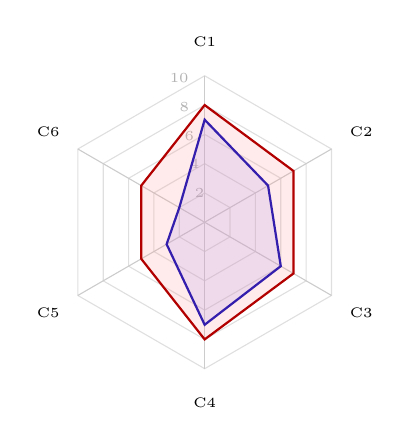
\begin{tikzpicture}[scale=0.62]
\pgfmathsetmacro{\R}{3}
\foreach \r in {0.6,1.2,1.8,2.4,3.0}{
  \draw[gray!25](90:\r)--(30:\r)--(-30:\r)--(-90:\r)--(-150:\r)--(150:\r)--cycle;}
\foreach \r/\v in {0.6/2,1.2/4,1.8/6,2.4/8,3.0/10}{
  \node[gray!60,font=\tiny] at (100:\r) {\v};}
\draw[gray!40](0,0)--(90:\R);
\draw[gray!40](0,0)--(30:\R);
\draw[gray!40](0,0)--(-30:\R);
\draw[gray!40](0,0)--(-90:\R);
\draw[gray!40](0,0)--(-150:\R);
\draw[gray!40](0,0)--(150:\R);
\node[font=\tiny] at (90:3.7)  {C1};
\node[font=\tiny] at (30:3.7)  {C2};
\node[font=\tiny] at (-30:3.7) {C3};
\node[font=\tiny] at (-90:3.7) {C4};
\node[font=\tiny] at (-150:3.7){C5};
\node[font=\tiny] at (150:3.7) {C6};
\draw[thick,blue!70!black,fill=blue!40,fill opacity=0.20]
  (90:2.1)--(30:1.5)--(-30:1.8)--(-90:2.1)--(-150:0.9)--(150:0.6)--cycle;
\draw[thick,red!70!black,fill=red!40,fill opacity=0.20]
  (90:2.4)--(30:2.1)--(-30:2.1)--(-90:2.4)--(-150:1.5)--(150:1.5)--cycle;
\end{tikzpicture}
\par\smallskip{\small\textbf{Famille C}}\par{\footnotesize Compétences métier}
\end{minipage}

\bigskip
\begin{center}
\textcolor{blue!70!black}{\rule{0.35cm}{0.35cm}}~\small Avant la formation (estimé)\qquad
\textcolor{red!70!black}{\rule{0.35cm}{0.35cm}}~\small Après la formation\qquad
\footnotesize Scores sur 10
\end{center}
\caption{Bilan de progression par famille de compétences (A, B, C) : autoévaluation avant/après formation.}
\end{figure}

\medskip

La lecture comparée des trois radars met en évidence plusieurs dynamiques que le texte seul ne suffit pas à rendre visibles.

\textbf{Sur la famille A (compétences sociales et personnelles)}, la surface bleue (avant formation) est clairement asymétrique : les dimensions A3 et A4 : capacité de réorientation et d'adaptation : étaient déjà relativement développées, adossées à une expérience professionnelle existante. En revanche, A1 et A5 restaient très en retrait, révélant un angle mort sur la diversification des méthodes et les démarches réflexives. La surface rouge (après formation) montre une expansion homogène et un rééquilibrage : les points faibles ont progressé davantage que les points forts, ce qui traduit un apprentissage ciblé plutôt qu'une simple consolidation de l'acquis.

\textbf{Sur la famille B (compétences méthodologiques)}, le radar illustre une asymétrie radicale dans mon point de départ : B4 (prototypage itératif) était à 2/10 : une lacune franche, pas une faiblesse relative : tandis que B6 (élaboration de roadmaps) constituait déjà une zone d'expertise à 7/10. La formation a permis de combler la lacune de B4 et d'harmoniser l'ensemble, sans écraser les acquis. Le fait que la surface rouge soit nettement plus régulière que la surface bleue signale précisément cela : moins de creux, moins de pics extrêmes, une posture méthodologique plus équilibrée.

\textbf{Sur la famille C (compétences métier)}, la forme bleue est caractéristique d'un profil d'expert sectoriel partiel : C1 et C4 sont élevés (ancrage dans l'expérience bancaire et professionnelle directe), mais C5 et C6 sont très faibles (angles morts sur les dimensions sociales et environnementales). La formation n'a pas tout résorbé : les scores après restent modestes sur C5--C6 : mais elle a rendu visible ce qui était invisible : ces zones ne sont plus des angles morts ignorés, elles sont devenues des axes de développement conscients et nommés.

\medskip
Les tableaux ci-dessous détaillent les scores et les justifications sous-jacentes à chacune de ces positions.

% -----------------------------------------------------------------------
% TABLEAUX DE DESCRIPTION
% -----------------------------------------------------------------------
\bigskip
\noindent\textbf{Famille A : Compétences sociales et personnelles}

\smallskip
\noindent\begin{tabularx}{\textwidth}{@{} c c c X @{}}
\toprule
\textbf{Dim.} & \textbf{Avant /10} & \textbf{Après /10} & \textbf{Justification de l'autoévaluation initiale} \\
\midrule
A1 & 3 & 6 & Difficultés marquées à diversifier les méthodes de travail. \\
A2 & 5 & 8 & Maîtrise partielle des approches agiles, mais compétences limitées en médiation et communication. \\
A3 & 6 & 7 & Bonne capacité à réorienter le groupe lorsqu'il est confronté à une impasse. \\
A4 & 5 & 7 & Aptitude correcte à ajuster l'approche lorsque la méthode initiale échoue. \\
A5 & 3 & 6 & Difficultés à mobiliser d'autres démarches réflexives. \\
A6 & 5 & 7 & Compétence effective mais seulement jusqu'à un certain niveau de complexité. \\
\bottomrule
\end{tabularx}

\bigskip
\noindent\textbf{Famille B : Compétences méthodologiques}

\smallskip
\noindent\begin{tabularx}{\textwidth}{@{} c c c X @{}}
\toprule
\textbf{Dim.} & \textbf{Avant /10} & \textbf{Après /10} & \textbf{Justification de l'autoévaluation initiale} \\
\midrule
B1 & 5 & 7 & Capacité à réaliser la tâche, mais avec un manque de méthodologie structurée. \\
B2 & 5 & 7 & Compétence correcte, nécessitant toutefois un approfondissement. \\
B3 & 4 & 6 & Approche globalement neutre. \\
B4 & 2 & 6 & Aucune expérience préalable de prototypage itératif. \\
B5 & 6 & 7 & Bonne aptitude à suivre une méthodologie, mais besoin d'en renforcer la maîtrise. \\
B6 & 7 & 8 & Expérience confirmée dans l'élaboration de roadmaps cohérentes et professionnelles. \\
\bottomrule
\end{tabularx}

\bigskip
\noindent\textbf{Famille C : Compétences métier}

\smallskip
\noindent\begin{tabularx}{\textwidth}{@{} c c c X @{}}
\toprule
\textbf{Dim.} & \textbf{Avant /10} & \textbf{Après /10} & \textbf{Justification de l'autoévaluation initiale} \\
\midrule
C1 & 7 & 8 & Expérience professionnelle dans le secteur bancaire, domaine du reporting transversal. \\
C2 & 5 & 7 & Compétence à tester et vérifier l'efficacité d'une synthèse. \\
C3 & 6 & 7 & Bonne capacité d'évaluation pour anticiper ce qui est fonctionnel ou non. \\
C4 & 7 & 8 & Expertise directement issue de l'activité professionnelle. \\
C5 & 3 & 5 & Connaissance limitée des impacts sociaux et environnementaux. \\
C6 & 2 & 5 & Maîtrise insuffisante des enjeux environnementaux. \\
\bottomrule
\end{tabularx}

\clearpage
\ClearShipoutPictureBG
